\documentclass{beamer}
\usepackage{graphicx}
\usepackage{tikz}
\usetikzlibrary{shapes,arrows}
\usepackage{tikz}
\usetheme{default}
%\usecolortheme{seahorse}
\usepackage{default}

  \setbeamertemplate{footline}[page number]
\setbeamertemplate{navigation symbols}{}
\setbeamertemplate{frametitle}[default][center]
\setbeamerfont{frametitle}{shape=\scshape}

\usepackage{color}

{\title{\textsc{Labor and Taxes Lecture}}
\author{Trevor S. Gallen}
\date{}



\begin{document}


\begin{frame}
\titlepage
\end{frame}

\begin{frame}
\frametitle[alignment=center]{Labor Supply/Demand Model}
\begin{itemize}
\item In this lecture, we'll try to understand the equilibrium labor model
\bigskip
\item It uses basic utility and production microeconomic models
\bigskip
\item You don't have to understand these on a deep level, and I'll try to give you a crash course
\bigskip
\item If you want more references, please ask
\end{itemize}
\end{frame}

\begin{frame}
\frametitle[alignment=center]{Labor Supply/Demand}
\begin{itemize}
\item Two sides of the market:  households supply labor and consume, firms demand labor and produce
\bigskip
\item Wages move to clear markets, so labor supplied is equal to labor demanded
\bigskip
\item Let's look at the household problem
\end{itemize}
\end{frame}

\begin{frame}
\frametitle[alignment=center]{Household problem}
\begin{itemize}
\item Households like two things:  they like consumption $c$ and leisure $\ell$, which we might write as total free time (normalized to one) minus labor hours $n$:
$$u(c,1-n)$$
\item Presumably, they always want more consumption and more labor:
$$\frac{\partial u}{\partial c}>0\ \ \ \frac{\partial u}{\partial \ell}>0$$
\item But have diminishing marginal utility from each:
$$\frac{\partial^2 u}{\partial c^2}<0\ \ \ \frac{\partial^2 u}{\partial \ell^2}<0$$
\item We can examine what we think their isoutility curves look like
\end{itemize}
\end{frame}

\begin{frame}
\frametitle[alignment=center]{Isoutility Curves}
\begin{figure}
 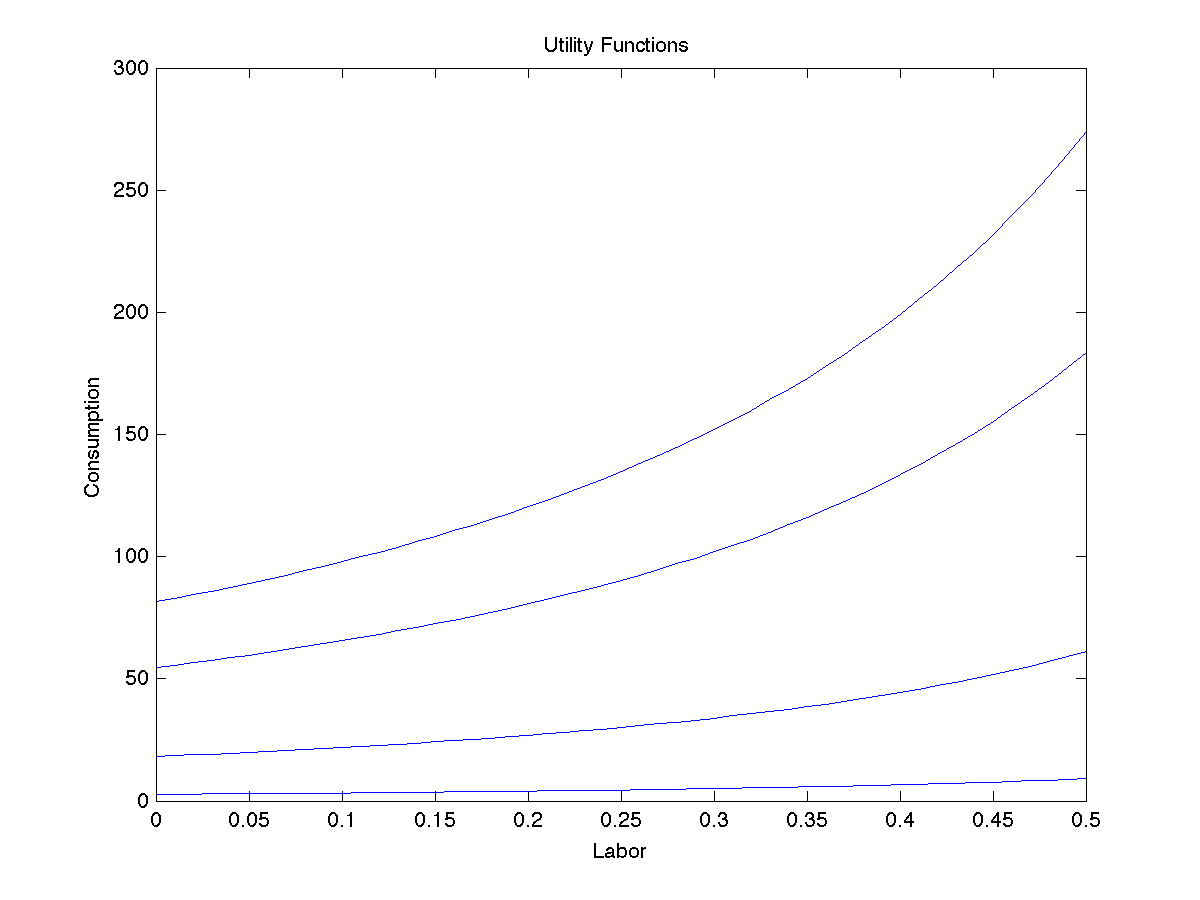
\includegraphics[scale=0.5]{Figure38.png}
\end{figure}
People are happier as they go to top left (more leisure, more consumption)
\end{frame}

\begin{frame}
\frametitle[alignment=center]{Household budget constraint}
\begin{itemize}
\item People want to maximize utility by choosing $c$ and $\ell$ (or $n$)
\bigskip
\item But how?  What's the tradeoff?
\bigskip
\item Budget constraint!  In simple world, consumption $c$ must equal wage per unit of time $w$ times amount of time worked $n$, plus any other income the household has $\nu$:
$$c=wn+\nu$$
\end{itemize}
\end{frame}

\begin{frame}
\frametitle[alignment=center]{Household Maximization Problem}
\begin{itemize}
\item Household wants to maximize $U(c,1-n)$ subject to the budget constraint
\bigskip
\item Maximization problem:
$$\mathcal{L}=U(c,1-n)+\lambda(wL+\nu-c)$$
They can maximize this by taking first-order conditions:
$$\frac{\partial \mathcal{L}}{\partial c}=0, \ \ \ \ \frac{\partial \mathcal{L}}{\partial n}=0$$
\item Which give:
$$\frac{\partial U}{\partial c}=\lambda$$
$$\frac{1}{w}\frac{\partial U}{\partial n}=\lambda$$
\item $\lambda$ is super important: if $\nu$ goes up by 1, $U$ goes up by $\lambda$
\end{itemize}
\end{frame}

\begin{frame}
\frametitle[alignment=center]{Household Maximization Problem}
$$\frac{\partial U}{\partial c}=\lambda$$
$$\frac{1}{w}\frac{\partial U}{\partial n}=\lambda$$
\begin{itemize}
\item $\lambda$ is the Lagrange multiplier:  value in terms of utility of another dollar (utility-dollar conversion rate) at margin
\item If you had another dollar from the sky, what could you do with it?  Two possibilities:
\begin{enumerate} 
\item Consume it, in which case you get $\frac{\partial U}{\partial c}$
\item Work less, in which case you buy $\frac{1}{w}$ fewer units of working and get $\frac{\partial U}{\partial n}$ utility per unit
\end{enumerate}
\item At margin, the two must be equal!
\end{itemize}
$$\frac{\partial U}{\partial c}=\frac{1}{w}\frac{\partial U}{\partial n}$$
or:
\small
$$\underbrace{\frac{\partial U}{\partial n}/\frac{\partial U}{\partial c}}_{\text{MRS}}=\underbrace{w}_{\text{MRTS}}$$
\end{frame}

\begin{frame}
\frametitle[alignment=center]{Household Maximization Problem}
$$\underbrace{\frac{\partial U}{\partial n}/\frac{\partial U}{\partial c}}_{\text{MRS}}=\underbrace{w}_{\text{MRTS}}$$
\begin{itemize}
\item Intuitively, what you get from trading off a unit of consumption for a unit of leisure (MRS) must equal the price (the wage/MRTS)
\bigskip
\item Fundamentally, this gives us an individual supply curve of labor: $\frac{\partial U}{\partial n}/\frac{\partial U}{\partial c}$ is really just a function of $n$ (because $c=wn+\nu$), $\nu$, and $U$.
\bigskip
\item As wage increases, can trace out labor supply curve
\bigskip
\item Let's give an example:
\end{itemize}
\end{frame}

\begin{frame}
\frametitle[alignment=center]{Labor Supply Curve: Example}
$$U(c,1-n)=\log(c)+\psi\log(8760-n)$$
\begin{itemize}
\item Free time/year = 24*365=8760
\item Where $\psi=2.5$, and $c=wn+\nu$, $\nu=8700$
\item Can solve for labor:
$$w=\frac{\nu  \psi }{8760-n (\psi +1)}$$
\item Let's graph it out!
\end{itemize}
\end{frame}

\begin{frame}
\frametitle[alignment=center]{Labor Supply Curve: Example}
\begin{figure}
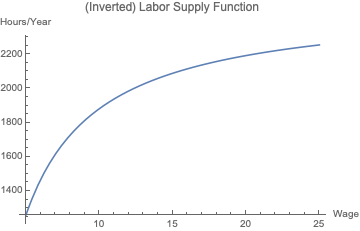
\includegraphics[scale=0.75]{LaborSupply1.png}
\end{figure}
\end{frame}

\begin{frame}
\frametitle[alignment=center]{Labor Supply Curve: Example}
\begin{figure}
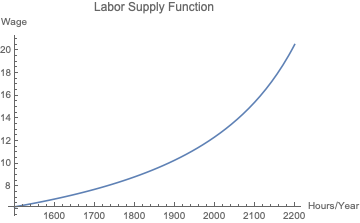
\includegraphics[scale=0.75]{LaborSupply2.png}
\end{figure}
\end{frame}

\begin{frame}
\frametitle[alignment=center]{Labor Supply Curve: Example}
\begin{figure}
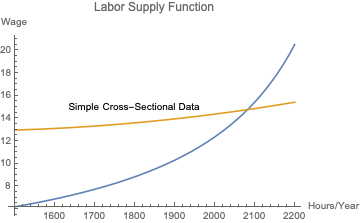
\includegraphics[scale=0.75]{LaborSupply3.png}
\end{figure}
If we include cross-sectional estimates (wrong!)
\end{frame}



\begin{frame}
\frametitle[alignment=center]{What about Labor Demand?}
\begin{itemize}
\item  We have our first labor supply curve...what about labor demand?
\bigskip
\item Imagine a firm that takes in labor $L$ and capital $K$ at per-unit costs $w$ and $r$
\bigskip
\item Produces $F(K,L)$, cost is $wL$ and $rK$.  Define profit $\pi$:
\bigskip
$$\pi=F(K,L)-wL-rK$$
\item Maximizes by choosing $K$ and $L$.  Let's focus on $L$
\end{itemize}
\end{frame}

\begin{frame}
\frametitle[alignment=center]{What about Labor Demand?}
$$\pi=F(K,L)-wL-rK$$
\ \\
$$\frac{\partial \pi}{\partial L}=0$$
or:\\
$$\frac{\partial F(K,L)}{\partial L}=w$$
\ \\
\begin{itemize}
\item Marginal benefit (amount produced when hire one more unit of labor) $\frac{\partial F(K,L)}{\partial L}$ equals marginal cost (wage, price paid for that extra unit) $w$
\item What do labor demand curves look like?
\end{itemize}
\end{frame}

\begin{frame}
\frametitle[alignment=center]{Labor Demand Curve: Example}
$$\pi=F(K,L)-wL-rK$$
\begin{itemize}
\item Let:
$$F(K,L)=AK^\alpha L^{1-\alpha}$$
\item so:
$$\frac{\partial F}{\partial L}=(1-\alpha) A\left(\frac{K}{L}\right)^\alpha$$
\item Productivity of $L$ is increasing in $K$ and decreasing in $L$
\item  Let's take a look!
 \end{itemize}
\end{frame}


\begin{frame}
\frametitle[alignment=center]{Isoproduction Curves}
\begin{figure}
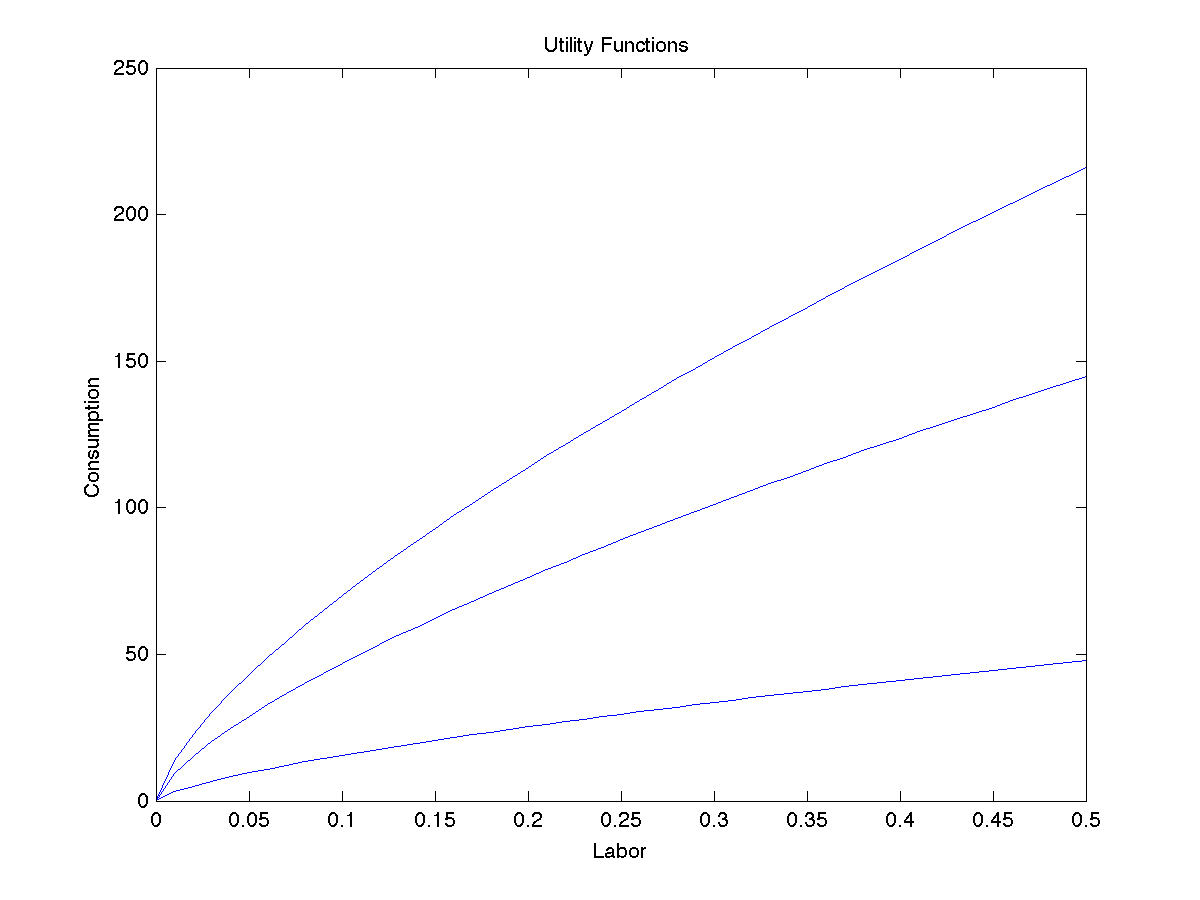
\includegraphics[scale=0.5]{Figure39.png}
\end{figure}
\end{frame}

\begin{frame}
\frametitle[alignment=center]{Labor demand curves, holding $K$ fixed}
\begin{figure}
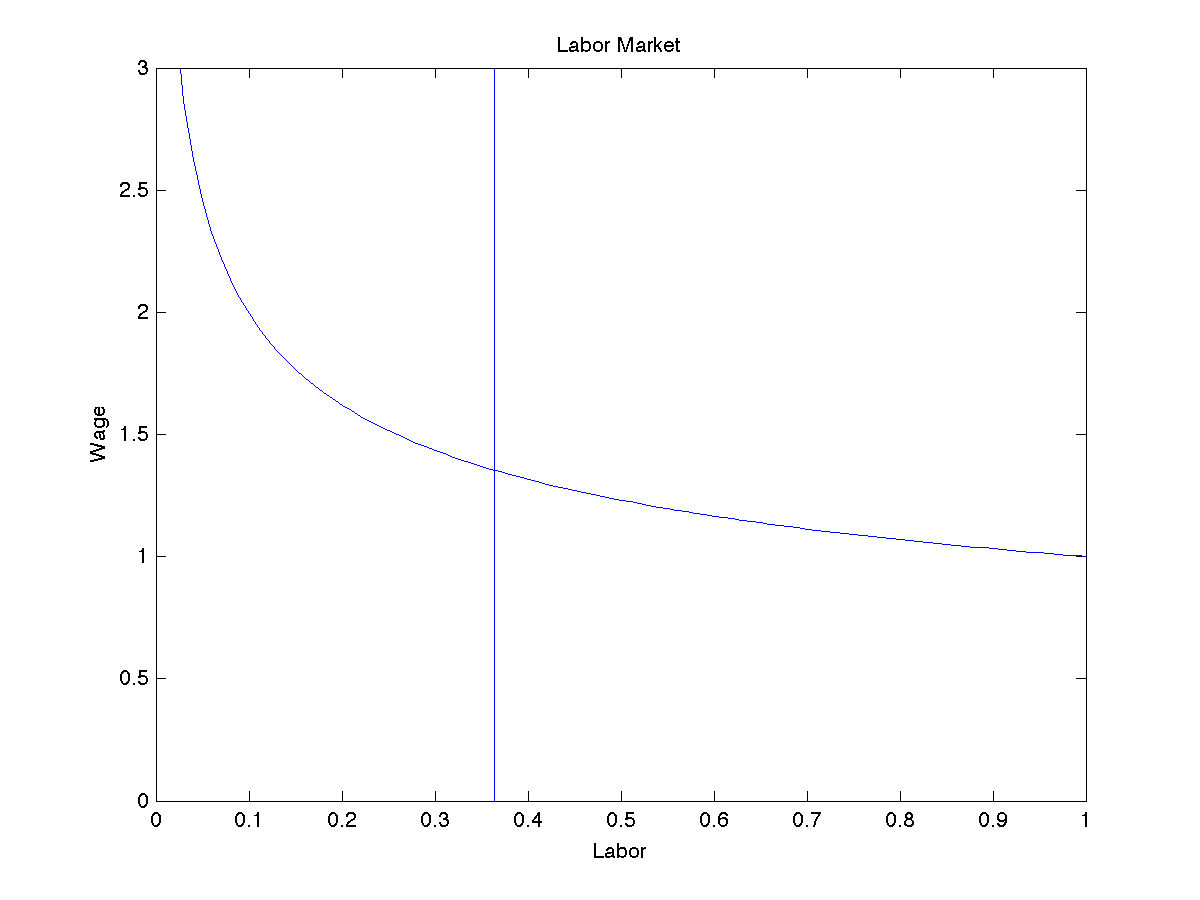
\includegraphics[scale=0.5]{Figure41.png}
\end{figure}
\end{frame}



\begin{frame}
\frametitle[alignment=center]{Labor Demand Curve: Example}
\begin{itemize}
\item Equilibrium is when both firm and household problems are satisfied
\bigskip
$$\frac{\frac{\partial U}{\partial n}}{\frac{\partial U}{\partial c}}=w$$
\item And:
$$\frac{\partial F(K,L)}{\partial L}=w$$
\item Gives, as an equliibrium condition:
$$\frac{\frac{\partial U}{\partial n}}{\frac{\partial U}{\partial c}}=\frac{\partial F(K,L)}{\partial L}$$
\item What does this look like in our isoutility/isoproduction framework?
\end{itemize}
\end{frame}


\begin{frame}
\frametitle[alignment=center]{Labor Market Equilibria }
\begin{figure}
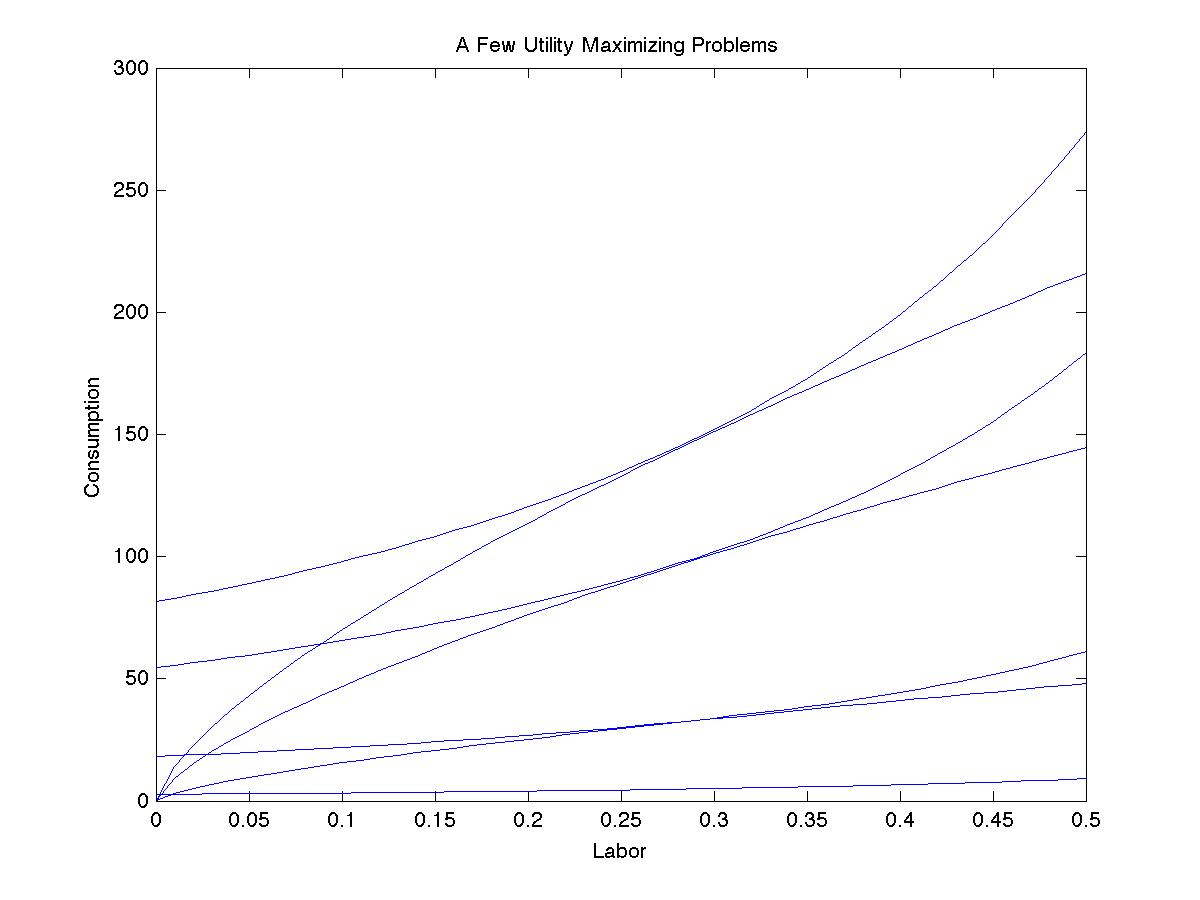
\includegraphics[scale=0.5]{Figure40.png}
\end{figure}
What about labor demand/supply?  Just put them together!
\end{frame}

\begin{frame}
\frametitle[alignment=center]{Note about preferences }
\begin{itemize}
\item Normally we use preferences like: $\log(c)+\psi\log(1-n)$
\item If you solve:
$$\mathcal{L}=\log(c)+\psi\log(1-n)$$
\item S.t. $c=wn$ (i.e. $\nu=0$) or if $\nu$ covaries 1-1 with $w$ then:
$$\frac{\partial \mathcal{L}}{\partial n}=\frac{w}{wn}-\frac{\psi}{1-n}=0$$
\item Or:
$$n^*=\frac{1}{1+\psi}$$
\item Labor demand is perfectly inelastic in this model!
\bigskip
\item But there's some evidence for this...
\end{itemize}
\end{frame}

\begin{frame}
\frametitle[alignment=center]{Inverted Labor Supply }
\begin{figure}
\centering
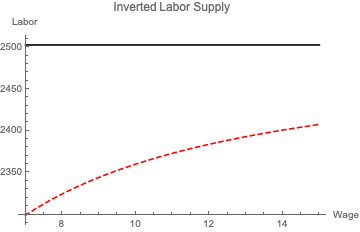
\includegraphics[scale=0.7]{LaborSupply6.png}
\end{figure}
$\nu=0$ vs $\nu=2000$
\end{frame}


\begin{frame}
\frametitle[alignment=center]{Labor Supply }
\begin{figure}
\centering
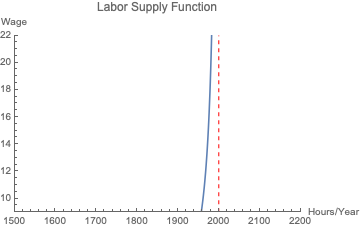
\includegraphics[scale=0.7]{LaborSupply4.png}
\end{figure}
\end{frame}

\begin{frame}
\frametitle[alignment=center]{Inelastic Labor Supply }
\begin{figure}
\centering
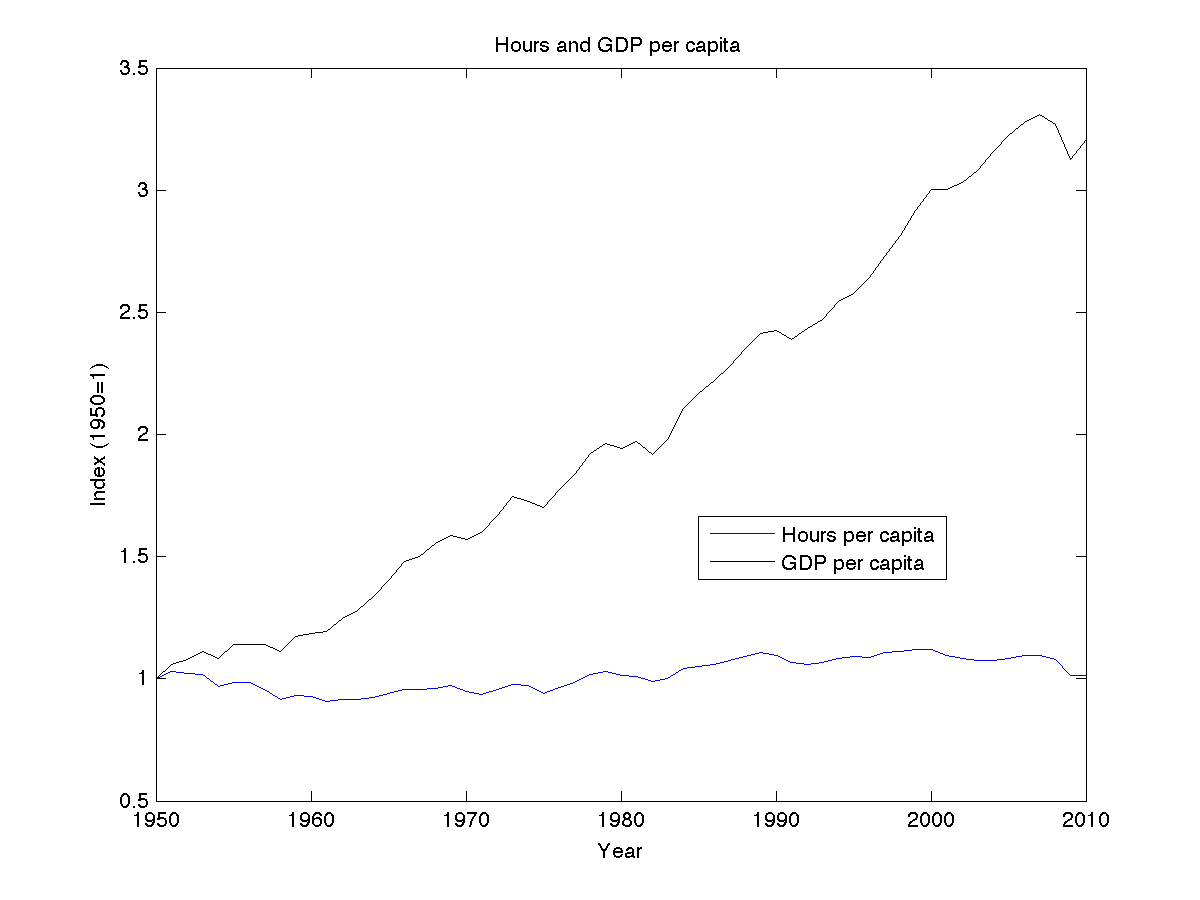
\includegraphics[scale=0.5]{Figure10.png}
\end{figure}
Okay, now let's put labor supply and demand together!
\end{frame}

\begin{frame}
\frametitle[alignment=center]{Supply and Demand }
\begin{figure}
\centering
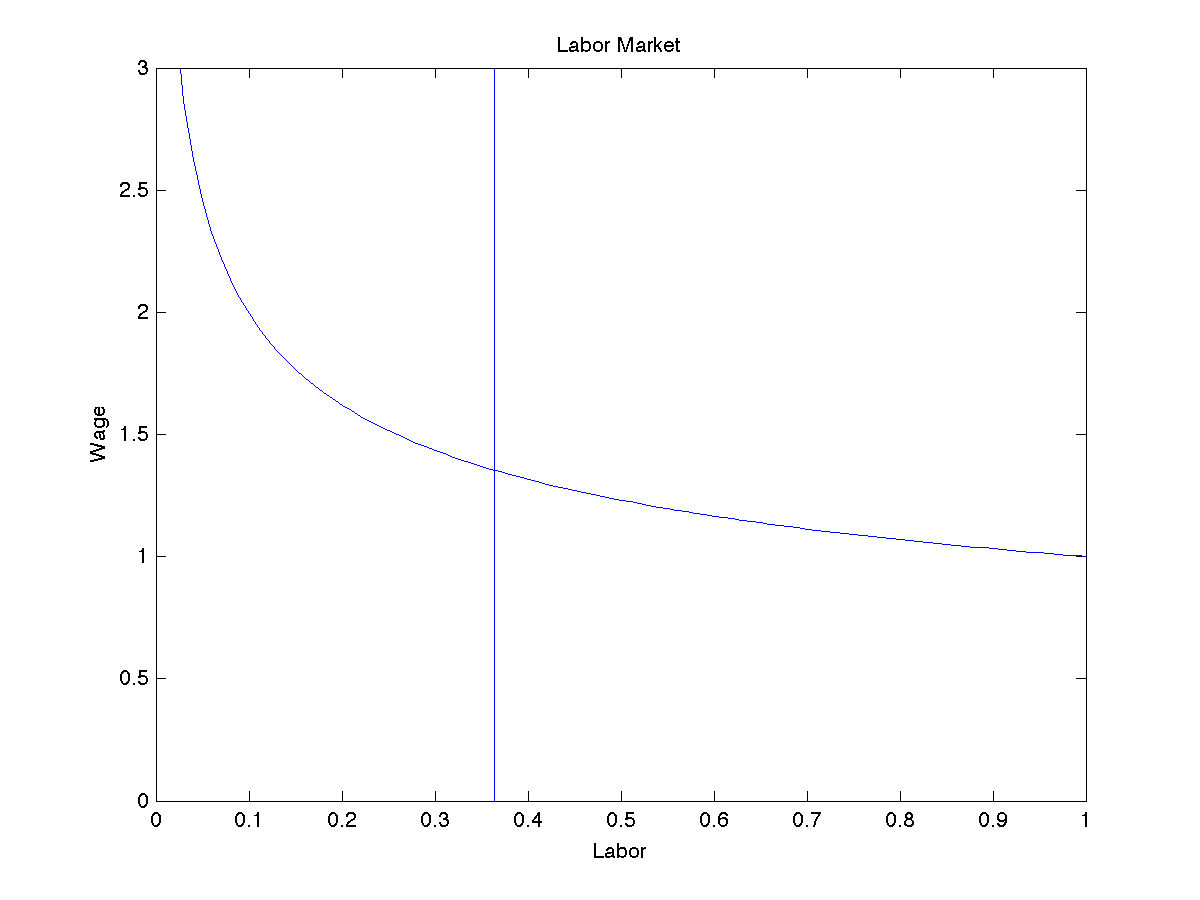
\includegraphics[scale=0.5]{Figure41.png}
\end{figure}
\end{frame}

\begin{frame}
\frametitle[alignment=center]{Inelastic Labor Supply }
\begin{itemize}
\item You can think of what I gave you as a bit like our ``long-run" model of supply and demand in labor markets.  
\bigskip
\item What happens when technology gets better (holding capital constant?)
\bigskip
\item What happens when capital increases (holding technology constant)?
\bigskip
\item What happens when we transfer more? (all else constant)
\end{itemize}
\end{frame}

\begin{frame}
\frametitle[alignment=center]{More Capital shifts Labor Demand }
\begin{figure}
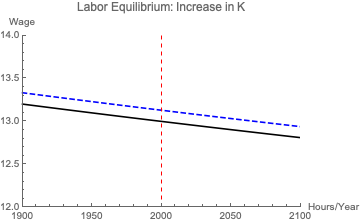
\includegraphics[scale=0.7]{MoreCapital.png}
\end{figure}
\end{frame}

\begin{frame}
\frametitle[alignment=center]{Higher TFP shifts Labor Demand }
\begin{figure}
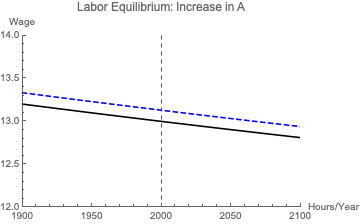
\includegraphics[scale=0.7]{MoreTFP.png}
\end{figure}
\end{frame}

\begin{frame}
\frametitle[alignment=center]{What about Taxes? }
\begin{itemize}
\item This is a public policy course isn't it?  Who cares about wages?
\bigskip
\item Taxes just affect wages.  Before, budget constraint was:
$$c=wn+\nu$$
\item With taxes, it's just:
$$(1+\tau^c)c=(1-\tau)wn+\nu-T$$
\item Where $\tau$ is the marginal tax rate and $T$ is transfer, lump-sum tax, (or possibly ``virtual income")
\item But we could have just written:
$$c=w^*n+\nu^*$$
\item Where $w^*=\frac{1-\tau}{1+\tau^c}$ and $\nu^*=\frac{\nu-T}{1+\tau^c}$
 \end{itemize}
\end{frame}


\begin{frame}
\frametitle[alignment=center]{What about Taxes on Firms? }
\begin{itemize}
\item Ordinary firm problem goes from:
$$\pi=F(K,L)-wL-rK$$
\item To:
$$\pi=F(K,L)-(1+\tau_L^F)wL-rK$$
\item Let's look at labor market equilibrium
 \end{itemize}
\end{frame}

\begin{frame}
\frametitle[alignment=center]{What about Taxes on Firms? }
\begin{itemize}
\item Ordinary firm problem goes from:
$$\pi=F(K,L)-wL-rK$$
\item To:
$$\pi=F(K,L)-(1+\tau_L^F)wL-rK$$
\item Let's look at labor market equilibrium
 \end{itemize}
\end{frame}

\begin{frame}
\frametitle[alignment=center]{Labor Market Equilibrium With Taxes }
\begin{itemize}
\item Labor market equilibrium:
$$\frac{\frac{\partial U}{\partial n}}{\frac{\partial U}{\partial c}}=\frac{\partial F(K,L)}{\partial L}$$
\item Changes to:
$$\frac{\frac{\partial U}{\partial n}}{\frac{\partial U}{\partial c}}=\frac{1-\tau}{(1+\tau_L^F)(1+\tau^c)}\frac{\partial F(K,L)}{\partial L}$$
\item All three taxes are really doing the same thing:  creating a wedge between what I get when I work and what I make when I work
\bigskip
\item When I give up an hour, all I care about is what I can eat with it, not if a lower leisure-consumption tradeoff comes from lower wage, higher labor taxes, or higher consumption taxes.
\bigskip
\item Also!  Important implication, it doesn't matter WHO is taxed!
 \end{itemize}
\end{frame}

\begin{frame}
\frametitle[alignment=center]{Tax Incidence - Irrelevancy }
\begin{figure}
\centering
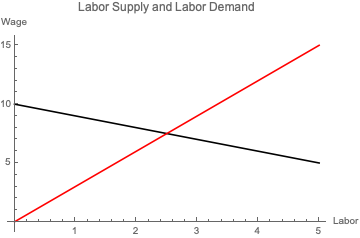
\includegraphics[scale=0.5]{TaxIncidence1.png}
 \end{figure}
\end{frame}

\begin{frame}
\frametitle[alignment=center]{Tax Incidence - Irrelevancy }
\begin{figure}
\centering
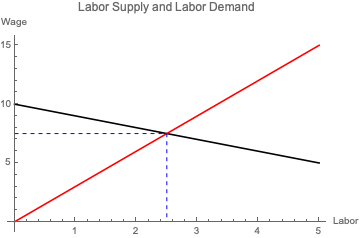
\includegraphics[scale=0.5]{TaxIncidence2.png}
 \end{figure}
\end{frame}

\begin{frame}
\frametitle[alignment=center]{Tax Incidence - Irrelevancy }
\begin{figure}
\centering
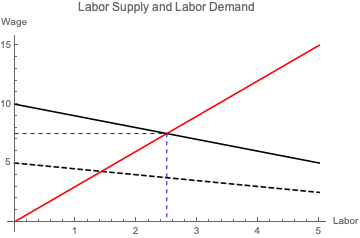
\includegraphics[scale=0.5]{TaxIncidence3.png}
 \end{figure}
\end{frame}

\begin{frame}
\frametitle[alignment=center]{Tax Incidence - Irrelevancy }
\begin{figure}
\centering
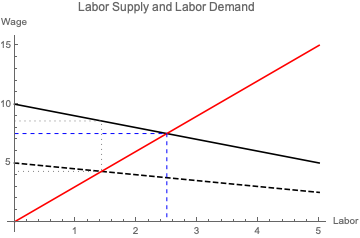
\includegraphics[scale=0.5]{TaxIncidence4.png}
 \end{figure}
\end{frame}

\begin{frame}
\frametitle[alignment=center]{Tax Incidence - Irrelevancy }
\begin{figure}
\centering
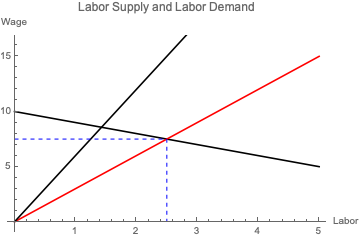
\includegraphics[scale=0.5]{TaxIncidence5.png}
 \end{figure}
\end{frame}

\begin{frame}
\frametitle[alignment=center]{Tax Incidence - Irrelevancy }
\begin{figure}
\centering
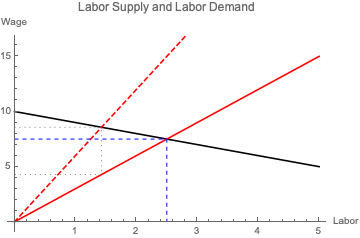
\includegraphics[scale=0.5]{TaxIncidence6.png}
 \end{figure}
\end{frame}

\begin{frame}
\frametitle[alignment=center]{Tax Incidence - Irrelevancy }
\begin{itemize}
\item Claim:  it doesn't matter who you statutorily put the tax on, the after-tax prices and quantities will be the same
\bigskip
\item BOLD
\bigskip
\item Where might we expect deviations?
\begin{itemize}
\item Tax avoidance
\item Minimum market prices
\end{itemize}
\item Let's look at some evidence
 \end{itemize}
\end{frame}

\begin{frame}
\frametitle[alignment=center]{Gasoline Tax }
\begin{itemize}
\item Doyle and Samphantharak 2008
\item IL and IN temporarily suspend gas taxes, then reinstate (political ploy)
\item Sales taxes formally fall on gas stations, not consumers
\item How do consumer prices respond? Will gas firms give consumers money out of the goodness of their hearts?
\begin{itemize}
\item Yes!(?)  
\end{itemize}
 \end{itemize}
\end{frame}

\begin{frame}
\frametitle[alignment=center]{Gasoline Tax }
\begin{figure}
\centering
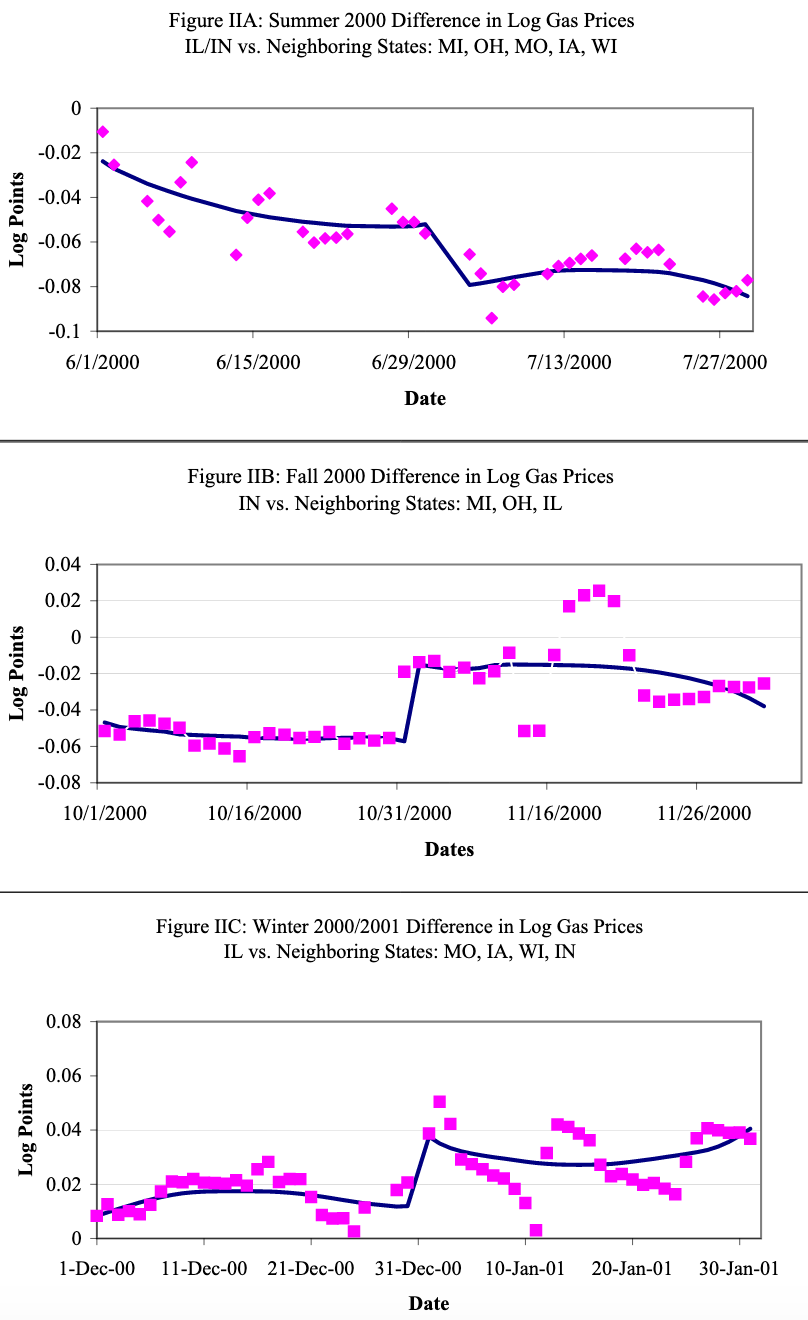
\includegraphics[scale=0.5]{DoyleSamphantharak2008.png} 
\end{figure}
70\% give tax, 100\% take tax (high pass-through)
\end{frame}

\begin{frame}
\frametitle[alignment=center]{EITC and Incidence Summary}
\begin{itemize}
\item Thinking through tax incidence is important!
\bigskip
\item Can't just tax firms and think it won't pass through to consumers: always on the pair
\bigskip
\item Nearly 100\% (sometimes estimated more) of cigarette taxes passed on to consumers (Evans, Ringel, Stech 1999)
\bigskip
\item Similarly, potentially 70\% of EITC goes to firms, not workers(!) (Rothstein 2010)
 \end{itemize}
\end{frame}



%\begin{frame}
%\frametitle[alignment=center]{Transfers Decrease Labor Supply }
%\begin{figure}
%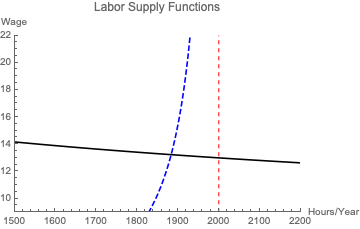
\includegraphics[scale=0.7]{LaborSupply7.png}
%\end{figure}
%\end{frame}

\begin{frame}
\frametitle[alignment=center]{Labor Supply}
\begin{itemize}
\item The fundamental models of labor supply macroeconomists use don't differ too greatly from this, just adds bells and whistles to make it more realistic, such as, for the family:
\begin{itemize}
\item Family labor supply (spousal labor and presence of children)
\smallskip
\item Discrete labor supply
\smallskip
\item Occupational/industrial choice
\smallskip
\item Taxes and transfers
\smallskip
\item Dynamic concerns, learning by doing, human capital
\smallskip
\item Health insurance, retirement
\end{itemize}
\item And for the firm:
\begin{itemize}
\item Many types of labor (high-skilled, low-skilled)
\smallskip
\item Taxes
\smallskip
\item Wage stickiness
\smallskip
\item Price stickiness
\smallskip
\item Matching frictions (fairly differnet)
\end{itemize}
\item And much, much more: but these are some core tradeoffs
\end{itemize}
\end{frame}

\begin{frame}
\frametitle[alignment=center]{Four Elasticities}
\begin{itemize}
\item There are four elasticities labor economists study and macroeconomists covet
\bigskip
\item I'll define them roughly
\begin{itemize}
\item Frisch (wage) elasticity of labor supply: how people respond  to temporary wage shocks
\item Hicksian (wage) elasticity of labor supply: how people respond to a tax+transfer
\item Marshallian (wage) elasticity of labor supply: how labor changes when wages increase forever
\item Income elasticity of labor supply:  how lifetime income falls when income (but not wage) increases
\end{itemize}
\item Note that these are all wrong: Frisch is elasticity holding marginal utility of income constant, Hicksian holds utility constant, and Marshallian is full derivative, but they capture household reactions
\item Sometimes people break these up into ``intensive" (hours/worker) and ``extensive" (\# workers) elasticities
\end{itemize}
\end{frame}

\begin{frame}
\frametitle[alignment=center]{Three Elasticities}
\begin{figure}
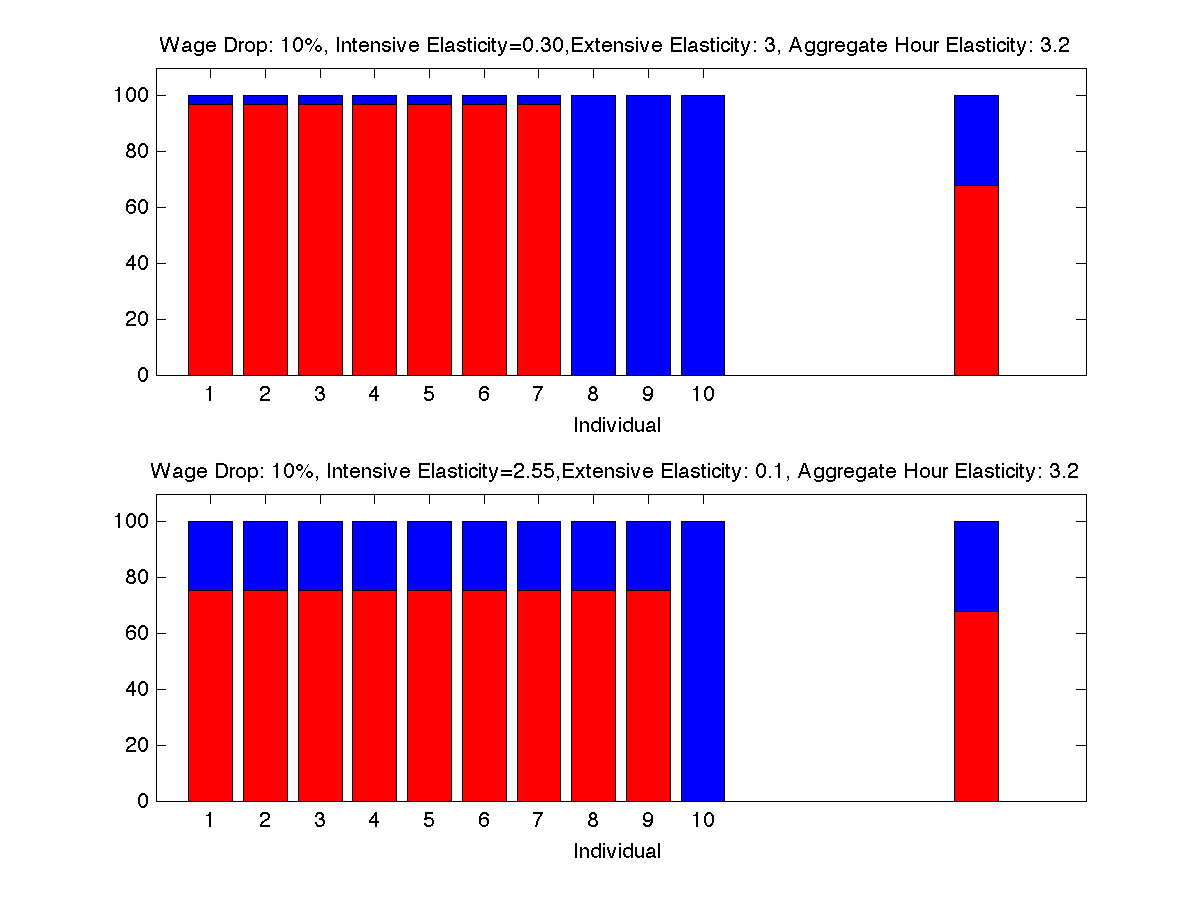
\includegraphics[scale=0.5]{Figure19.png}
\end{figure}
Two ways of getting an aggregate elasticity
\end{frame}

\begin{frame}
\frametitle[alignment=center]{Three Elasticities}
\begin{figure}
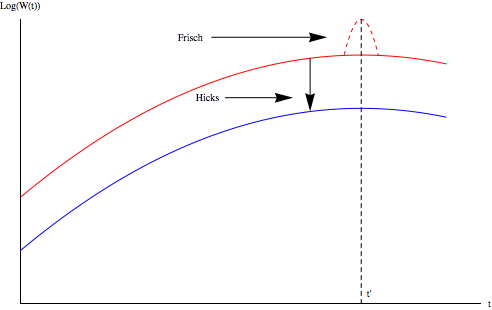
\includegraphics[scale=0.5]{Figure20.png}
\end{figure}
Frisch vs Hicksian
\end{frame}

\begin{frame}
\frametitle[alignment=center]{Three Elasticities}
\begin{figure}
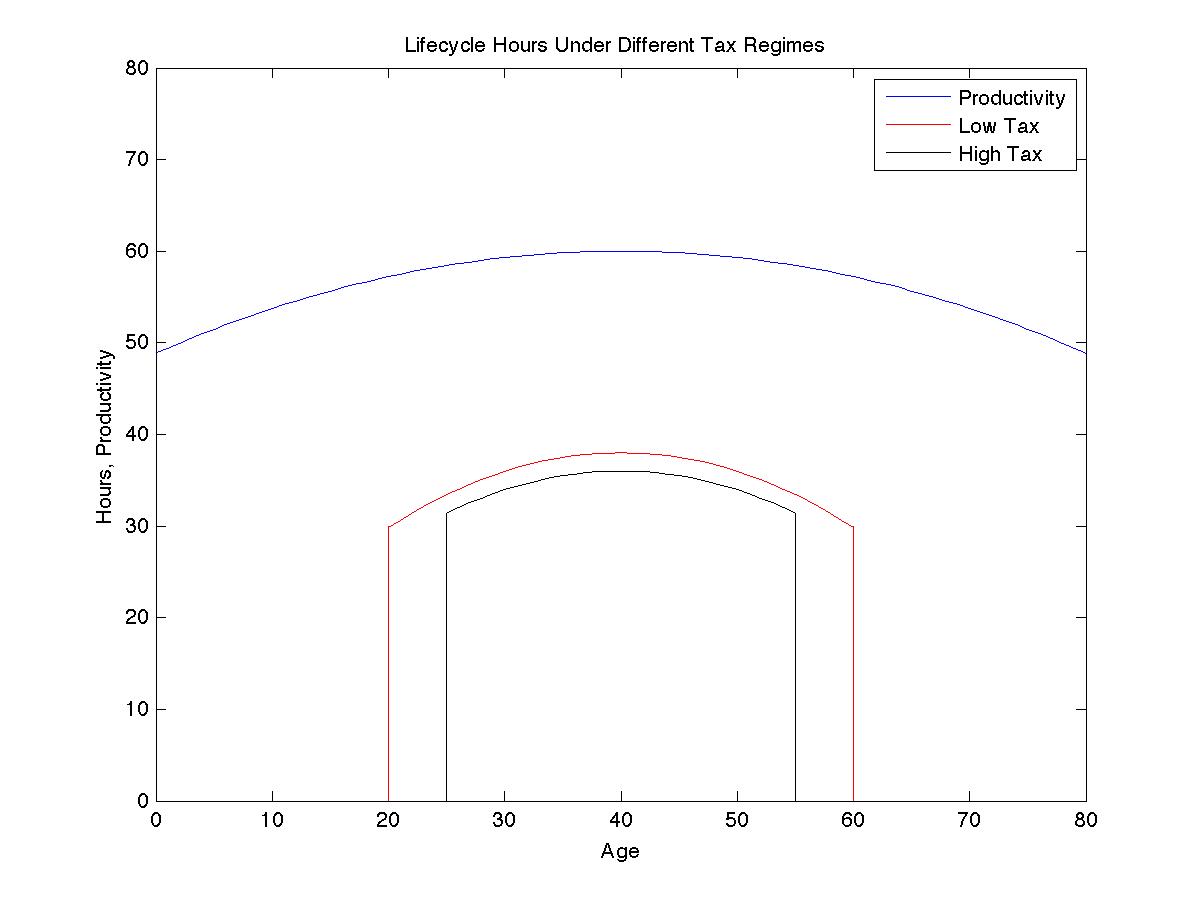
\includegraphics[scale=0.5]{Figure21.png}
\end{figure}
Example of extensive elasticity via retirement
\end{frame}

\begin{frame}
\frametitle[alignment=center]{Blundell, Bozio, Laroque}
\begin{figure}
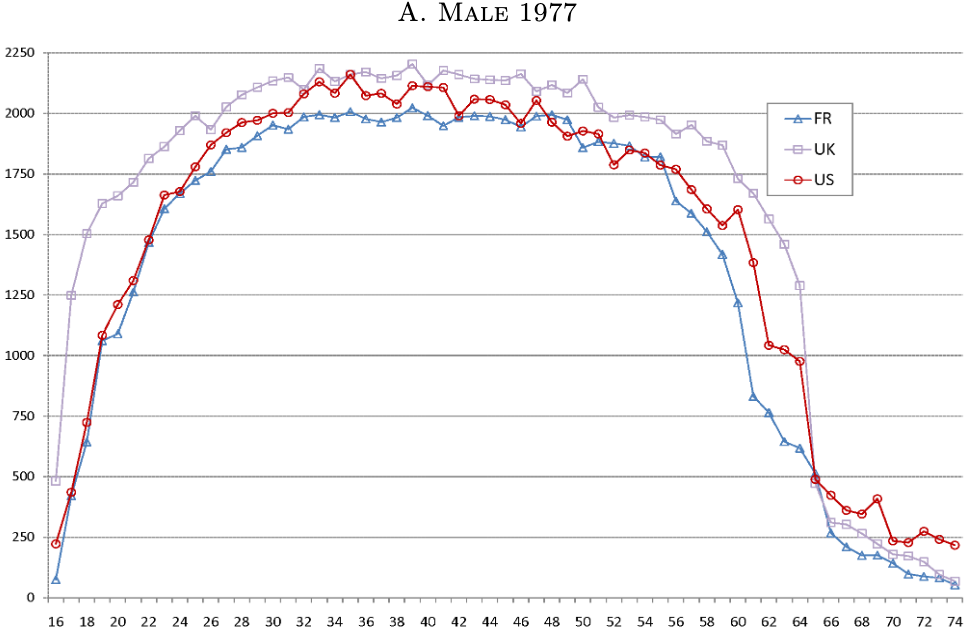
\includegraphics[scale=0.63]{Male1977.png}
\end{figure}
\end{frame}

\begin{frame}
\frametitle[alignment=center]{Blundell, Bozio, Laroque}
\begin{figure}
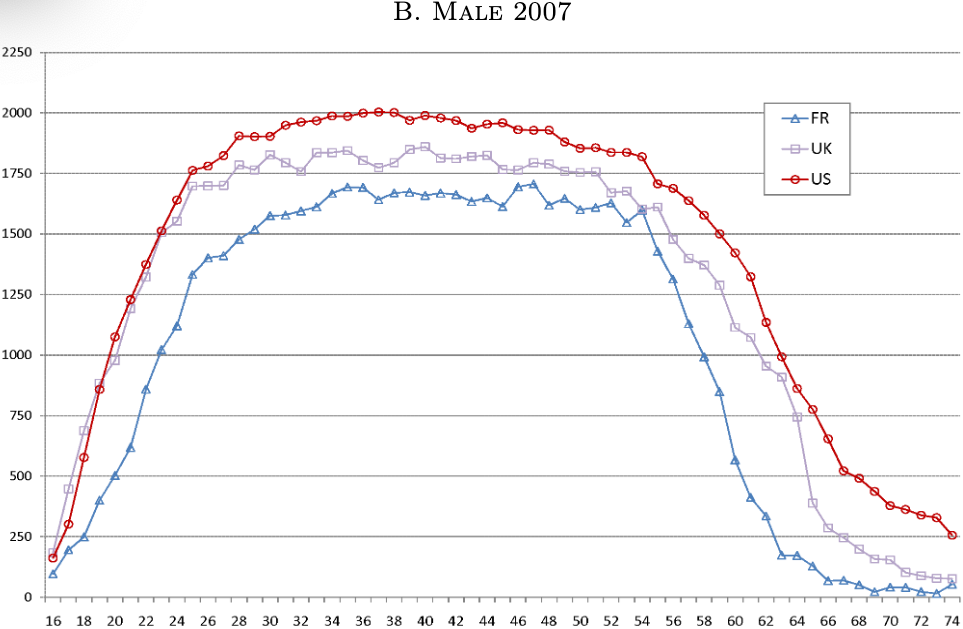
\includegraphics[scale=0.63]{Male2007.png}
\end{figure}
\end{frame}

\begin{frame}
\frametitle[alignment=center]{Blundell, Bozio, Laroque}
\begin{figure}
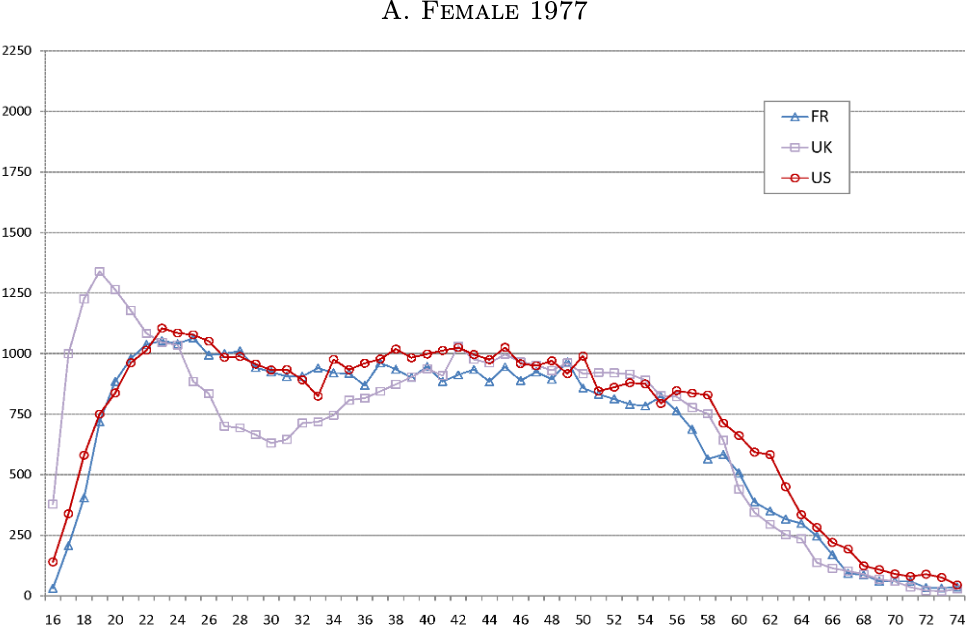
\includegraphics[scale=0.63]{Female1977.png}
\end{figure}
\end{frame}

\begin{frame}
\frametitle[alignment=center]{Blundell, Bozio, Laroque}
\begin{figure}
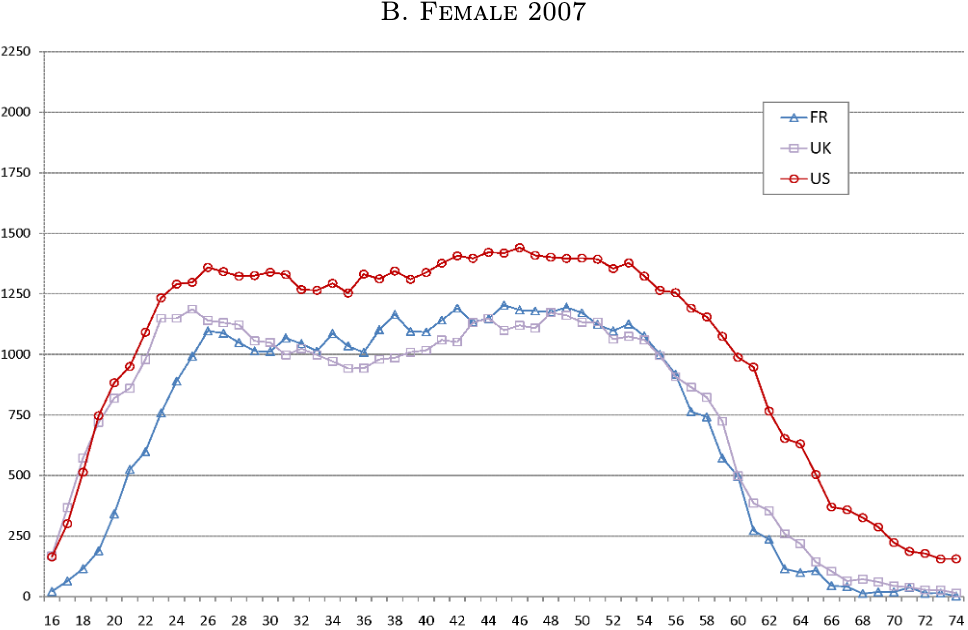
\includegraphics[scale=0.63]{Female2007.png}
\end{figure}
\end{frame}

\begin{frame}
\frametitle[alignment=center]{Estimates}
\begin{itemize}
\item In case you're curious about estimated elasticities
\bigskip
\item Enormous controversy about all
\bigskip
\item But what I find most convincing for aggregate hours:
\begin{itemize}
\item Frisch:  -0.75
\item Hicksian: -0.5
\item Income: -0.15
\item Marshallian: 0 to -0.2
\end{itemize}
\item Some disagree!
\end{itemize}
\end{frame}

\begin{frame}
\frametitle[alignment=center]{Income Effect: Lottery}
\begin{figure}
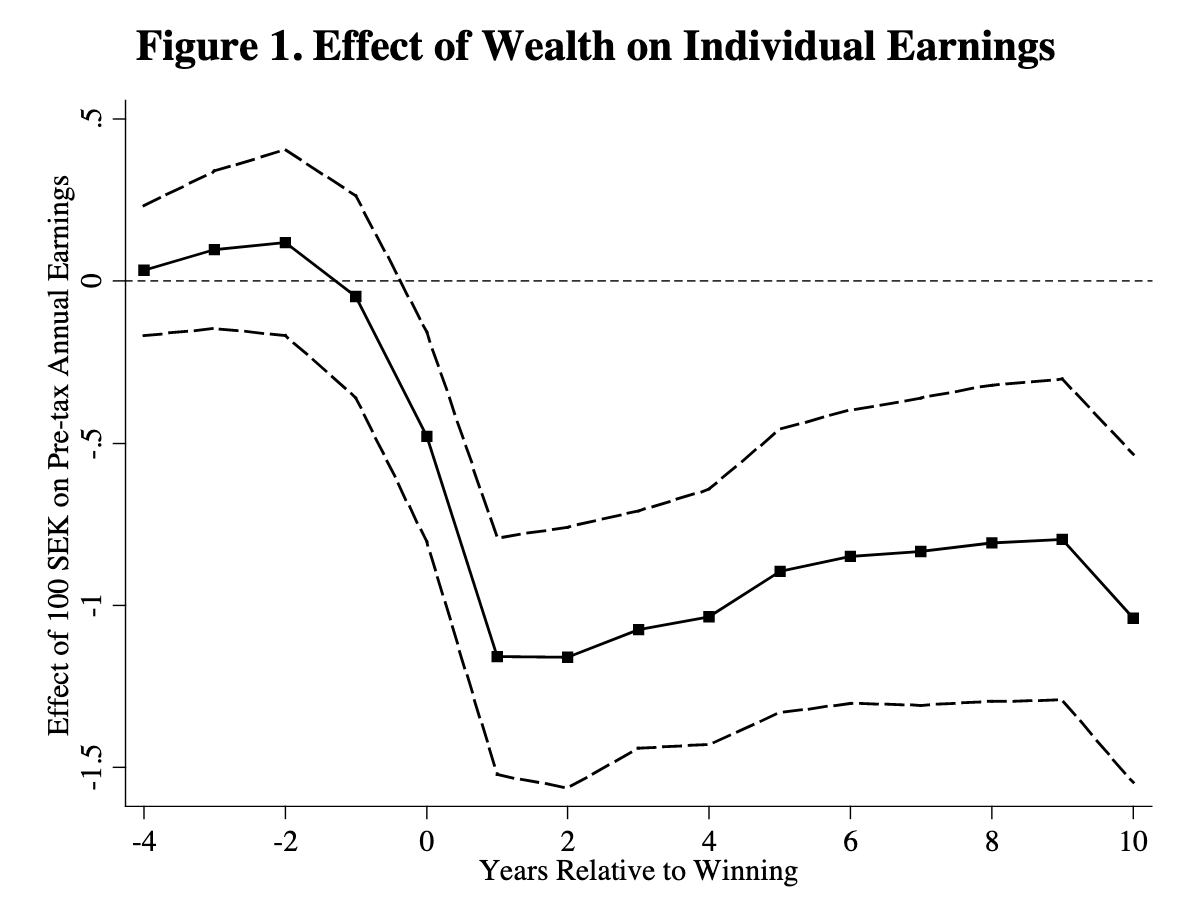
\includegraphics[scale=0.5]{CesariniNoto.png}
\end{figure}
\end{frame}


\begin{frame}
\frametitle[alignment=center]{Income Effect: Lottery}
\begin{figure}
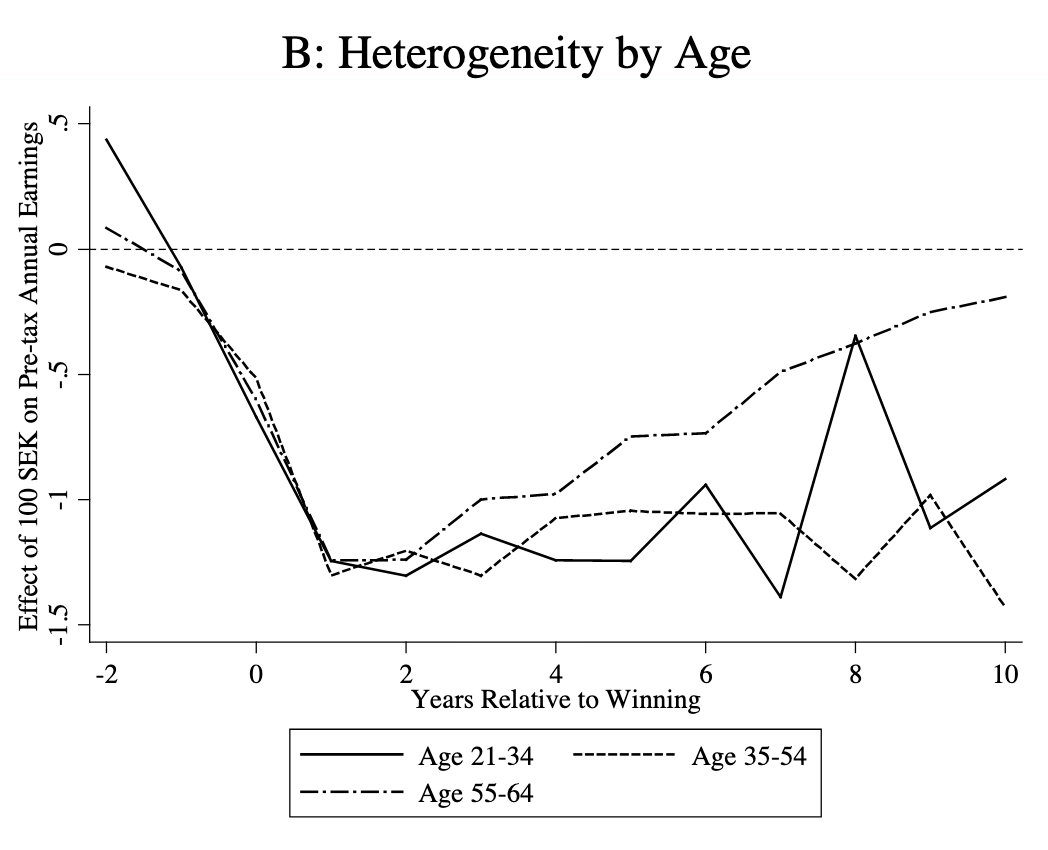
\includegraphics[scale=0.5]{CesariniNoto2.png}
\end{figure}
\end{frame}

\begin{frame}
\frametitle[alignment=center]{Prescott 2004: Hicksian Elasticities}
\begin{figure}
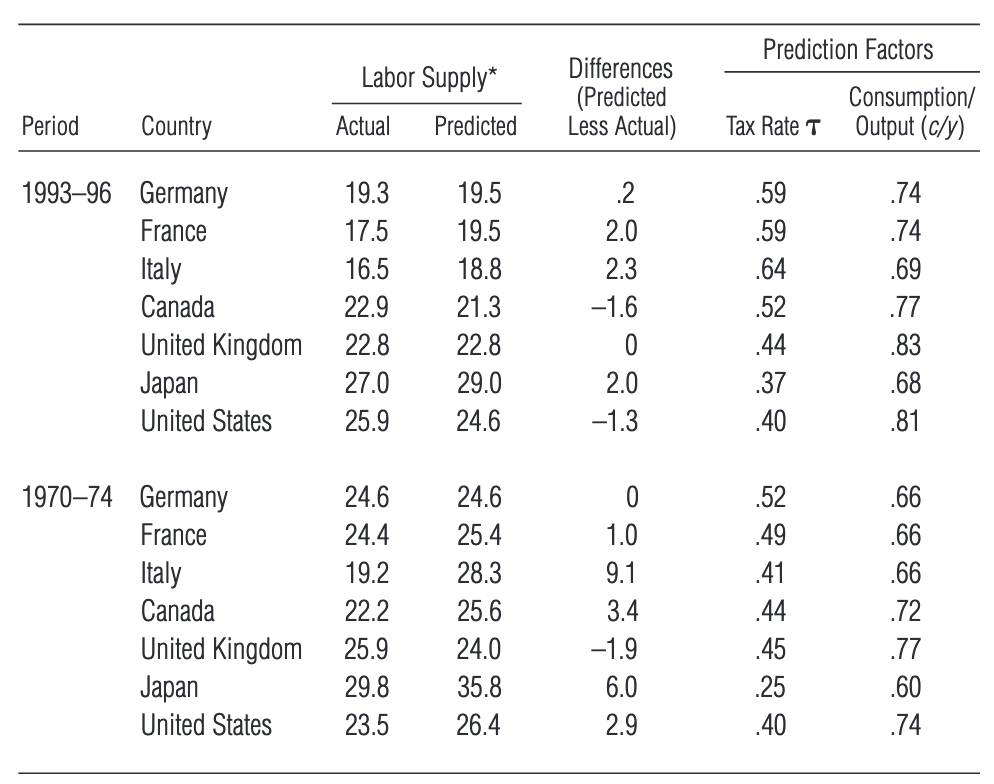
\includegraphics[scale=0.5]{Prescott2004.png}
\end{figure}
\end{frame}

\begin{frame}
\frametitle[alignment=center]{Prescott 2004: Hicksian Elasticities}
\begin{figure}
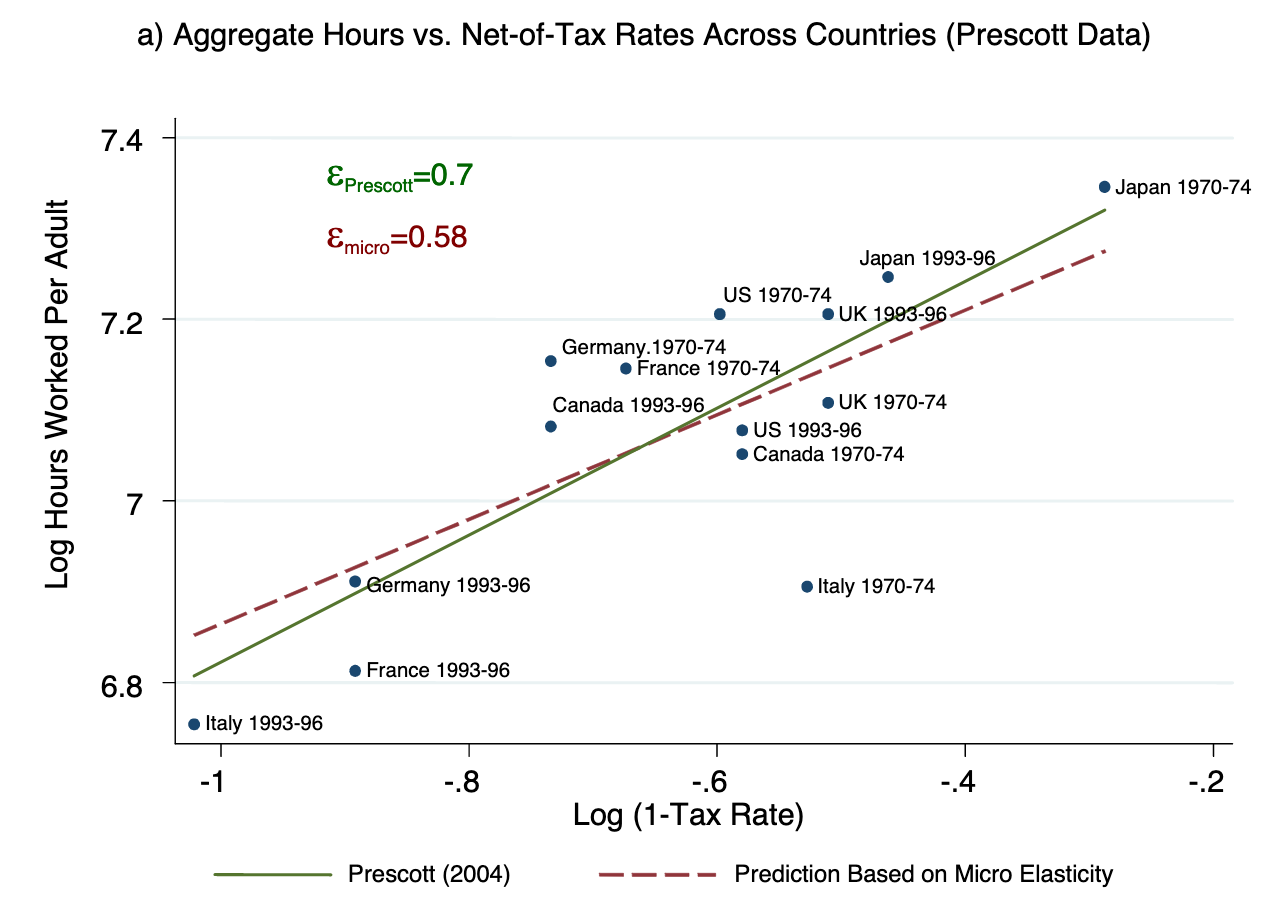
\includegraphics[scale=0.5]{Chettyx.png}
\end{figure}
From Chetty et al 2012
\end{frame}


\begin{frame}
\frametitle[alignment=center]{Chetty 2012}
\begin{itemize}
\item There's a weird disconnect between micro studies and macro studies
\bigskip
\item Chetty (2012) proposes it's because one is long-run/large variation (macro) and the other is small changes 
\bigskip
\item Big differences if there are optimization frictions
\bigskip
\item How big do optimization frictions on hours have to be to reconcile the literatures?
\end{itemize}
\end{frame}

\begin{frame}
\frametitle[alignment=center]{Chetty 2012}
\begin{figure}
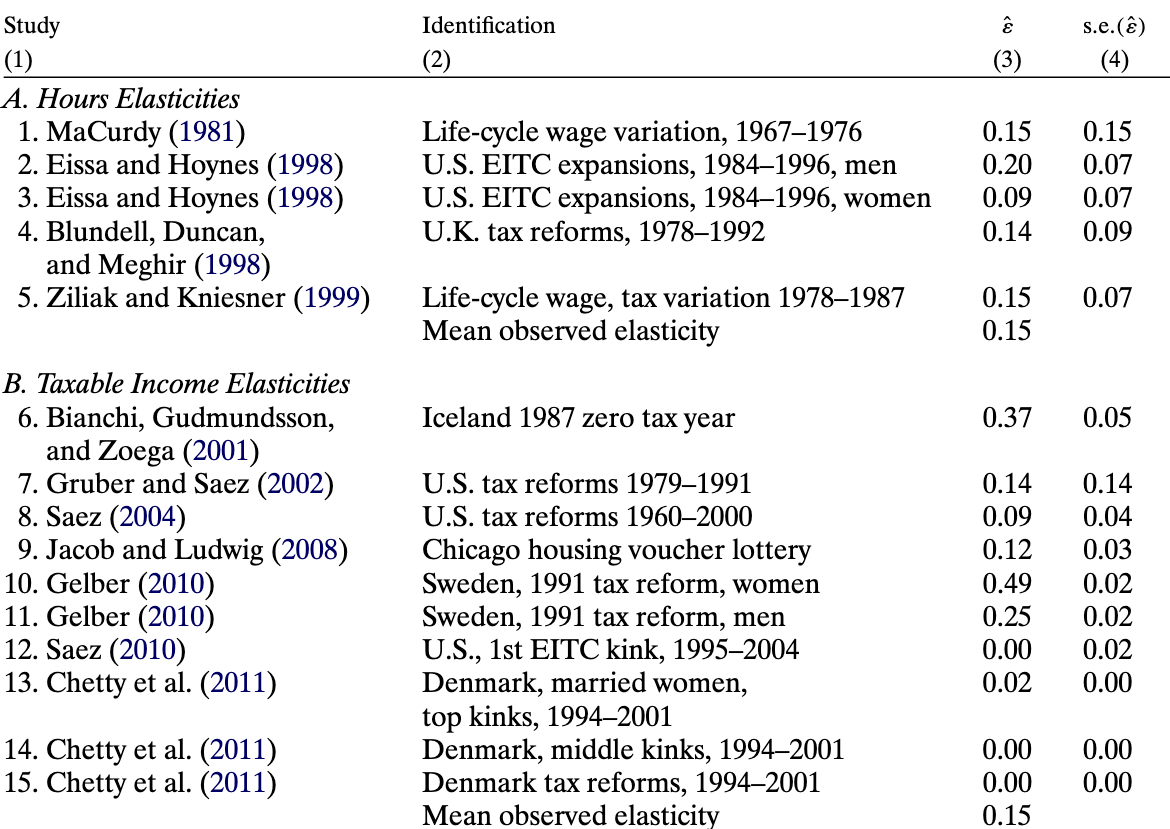
\includegraphics[scale=0.5]{Chetty2.png}
\end{figure}
\end{frame}

\begin{frame}
\frametitle[alignment=center]{Chetty 2012}
\begin{figure}
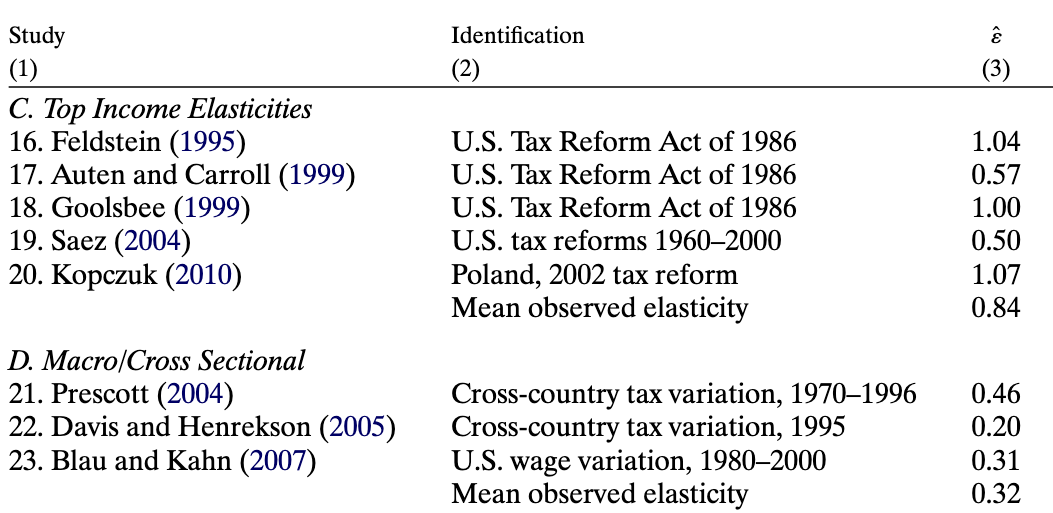
\includegraphics[scale=0.5]{Chetty3.png}
\end{figure}
\end{frame}


\begin{frame}
\frametitle[alignment=center]{Chetty 2012}
\begin{figure}
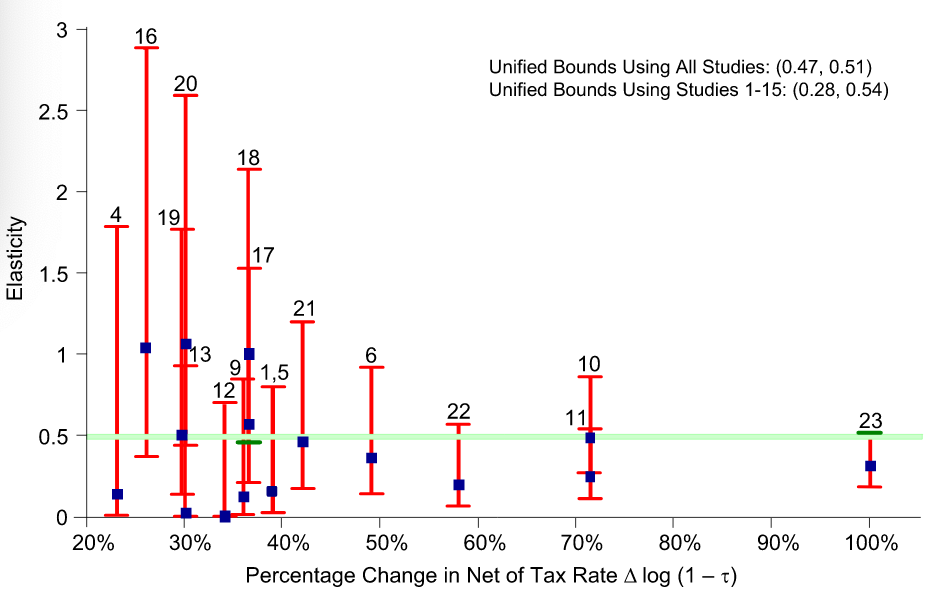
\includegraphics[scale=0.7]{Chetty1.png}
\end{figure}
\end{frame}


\begin{frame}
\frametitle[alignment=center]{Chetty 2012}
\begin{itemize}
\item There's a weird disconnect between micro studies and macro studies
\bigskip
\item Chetty (2012) proposes it's because one is long-run/large variation (macro) and the other is small changes 
\bigskip
\item Big differences if there are optimization frictions
\bigskip
\item How big do optimization frictions on hours have to be to reconcile the literatures?
\end{itemize}
\end{frame}


\begin{frame}
\frametitle[alignment=center]{Bianci et al 2001}
\begin{itemize}
\item Before 1988, Iceland taxed this year's income depending on last year's 
\bigskip
\item Normally, pay tax from 1986 in 1987's income, 1988 with tax base of 1987
\bigskip
\item But switched in 1988, so in 1987, never pay taxes on 1987 income (1986 in 1987, 1988 in 1988).
\bigskip
\item ``Tax-free" year (but still paying taxes, just not punished for earning more)
\end{itemize}
\end{frame}


\begin{frame}
\frametitle[alignment=center]{Bianci et al 2001: Frisch Elasticities}
\begin{figure}
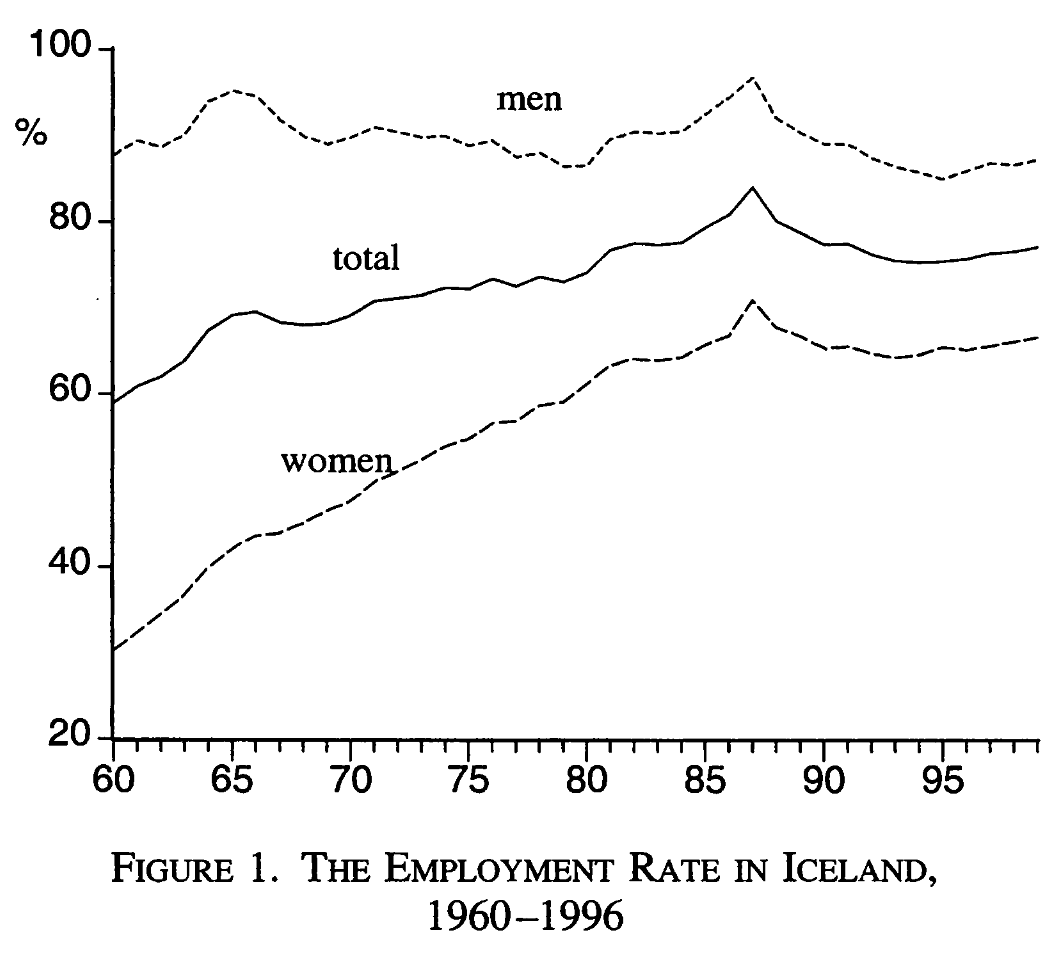
\includegraphics[scale=0.5]{Iceland_1.png}
\end{figure}
\end{frame}

\begin{frame}
\frametitle[alignment=center]{Bianci et al 2001: Frisch Elasticities}
\begin{figure}
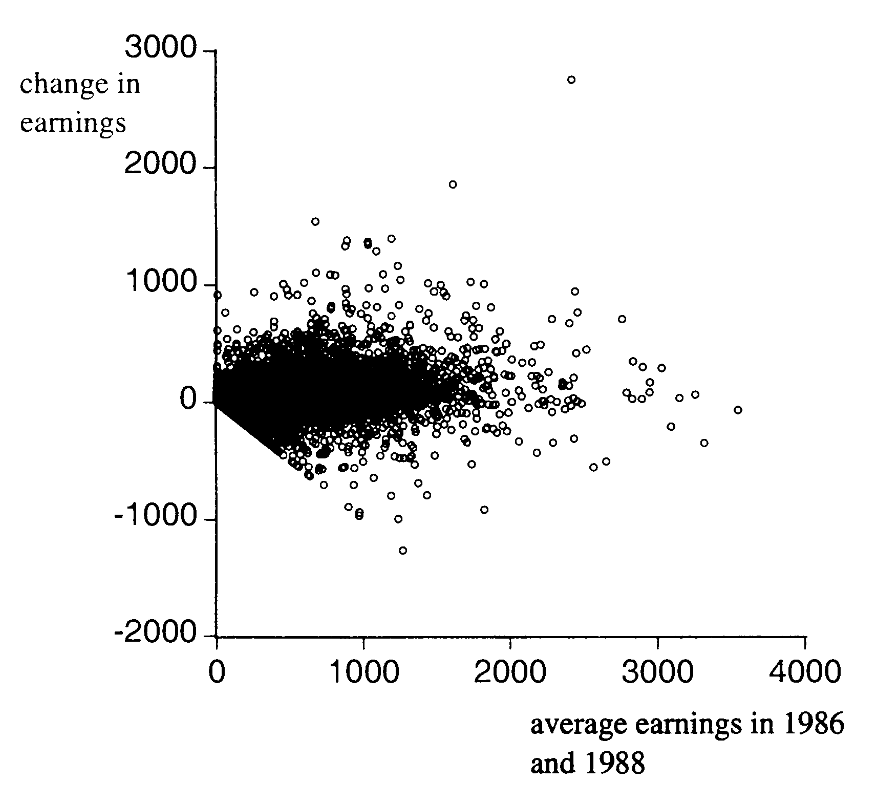
\includegraphics[scale=0.7]{Iceland_2.png}
\end{figure}
\end{frame}

\begin{frame}
\frametitle[alignment=center]{Bianci et al 2001: Frisch Elasticities}
\begin{figure}
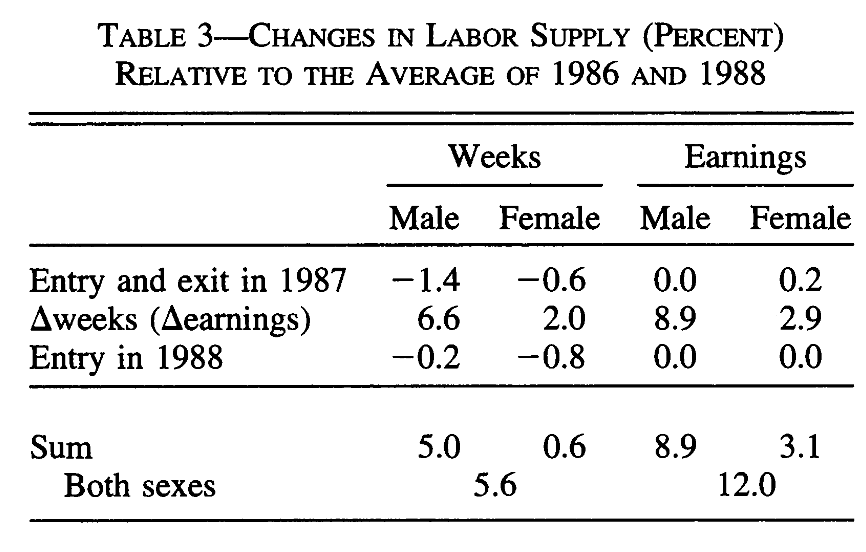
\includegraphics[scale=0.7]{Iceland_3.png}
\end{figure}
Elasticity of male earnings of 0.8, much from extensive margin.
\end{frame}

\begin{frame}
\frametitle[alignment=center]{Takeaways}
\begin{itemize}
\item It's easy to think theoretical labor econ is stupid...
\bigskip
\item It isn't!
\bigskip
\item My read: we've moved toward consensus, importance of ``intensive" vs ``extensive" and who (young/elderly, women) and optimization frictions
\end{itemize}
\end{frame}





\end{document}